% !TeX spellcheck = en_US
% Dieses Dokument muss mit PDFLatex gesetzt werden
% Vorteil: Grafiken koennen als jpg, png, ... verwendet werden
%          und die Links im Dokument sind auch gleich richtig
%
%Ermöglicht \\ bei der Titelseite (z.B. bei supervisor)
%Siehe https://github.com/latextemplates/uni-stuttgart-cs-cover/issues/4
\RequirePackage{kvoptions-patch}

%Englisch:
\let\ifdeutsch\iffalse
\let\ifenglisch\iftrue{}

%Deutsch:
%\let\ifdeutsch\iftrue
%\let\ifenglisch\iffalse

%
\ifdeutsch
	\PassOptionsToClass{numbers=noenddot}{scrbook}
\fi

%Warns about outdated packages and missing caption delcarations
%See https://www.ctan.org/pkg/nag
\RequirePackage[l2tabu, orthodox]{nag}

%Neue deutsche Trennmuster
%Siehe http://www.ctan.org/pkg/dehyph-exptl und http://projekte.dante.de/Trennmuster/WebHome
%Nur für pdflatex, nicht für lualatex
\RequirePackage{ifluatex}
\ifluatex
%do not load anything
\else
	\ifdeutsch
		\RequirePackage[ngerman=ngerman-x-latest]{hyphsubst}
	\fi
\fi

\documentclass[
               fontsize=12pt, %Default: 11pt, bei Linux Libertine zu klein zum Lesen
% BEGINN: Optionen für typearea
               paper=a4,
               twoside, % fuer die Betrachtung am Schirm ungeschickt
               BCOR=3mm, % Hack für BCOR (1.92 o.ä.), da bei BCOR2mm die Fuellpunkte beim Inhaltsverzeichnis falsch sind. Hack aber nicht mehr nötig: microtype für Verzeichnisse ausschalten hilft.
               DIV=13,   % je höher der DIV-Wert, desto mehr geht auf eine Seite. Gute werde sind zwischen DIV=12 und DIV=15
               headinclude=true,
               footinclude=false,
% ENDE: Optionen für typearea
%               titlepage,
               bibliography=totoc,
%               idxtotoc,   %Index ins Inhaltsverzeichnis
%                liststotoc, %List of X ins Inhaltsverzeichnis, mit liststotocnumbered werden die Abbildungsverzeichnisse nummeriert
               headsepline,
               cleardoublepage=empty,
               parskip=half,
%               draft    % um zu sehen, wo noch nachgebessert werden muss - wichtig, da Bindungskorrektur mit drin
               final   % ACHTUNG! - in pagestyle.tex noch Seitenstil anpassen
               ]{scrbook}

%%%
% Beschreibung:
% In dieser Datei werden zuerst die benoetigten Pakete eingebunden und
% danach diverse Optionen gesetzt. Achtung Reihenfolge ist entscheidend!
%
%%%


%%%
% Styleguide:
%
% Ein sehr kleiner Styleguide. Packages werden in Blöcken organisiert.
% Ein Block beginnt mit drei % in einer Zeile, dann % <Blocküberschrift>, dann
% eine Liste der möglichen Optionen und deren Einstellungen, Gründe und Kommentare
% eine % Zeile in der sonst nichts steht und dann wieder %%% in einer Zeile.
%
% Zwischen zwei Blöcken sind 2 Leerzeilen!
% Zu jedem Paket werden soviele Optionen wie möglich/nötig angegeben
%
%%%


%%%
% Codierung
% Wir sind im 21 Jahrhundert, utf-8 löst so viele Probleme.
%
% Mit UTF-8 funktionieren folgende Pakete nicht mehr. Bitte beachten!
%   * fancyvrb mit §
%   * easylist -> http://www.ctan.org/tex-archive/macros/latex/contrib/easylist/
\ifluatex
%no package loading required
\else
\usepackage[utf8]{inputenc}
\fi
%
%%%


%%%
% Deckblattstyle
%
\ifdeutsch
\PassOptionsToPackage{language=german}{uni-stuttgart-cs-cover}
\else
\PassOptionsToPackage{language=english}{uni-stuttgart-cs-cover}
\fi

\newcommand{\docauthor}{Raghuraj Tarikere Phaniraja Setty}
\newcommand{\doctitle}{Space Component Model using DLR Software Technologies}

\usepackage[
title={\doctitle},
author={\docauthor},
type=master,
institute=isterss,
number=12345,
course=se,
examiner={Dr.-Ing.\ Andr\'{e} van Hoorn (Prof.-Vertr.)},
supervisor={Dr.\ Du\v{s}an Okanovi\'{c},\\Teerat Pitakrat,\ M.Sc.},
startdate={October 2, 2017}, % English: July 5, 2013;    ISO: 2013-07-05
enddate={April 2, 2018}, % English: January 5, 2014; ISO: 2014-01-05
crk={I.7.2}
]{uni-stuttgart-cs-cover}
%
%%%


%%%
%Parallelbetrieb tex4ht und pdflatex
\makeatletter
\@ifpackageloaded{tex4ht}{\def\iftex4ht{\iftrue}}
                         {\def\iftex4ht{\iffalse}}
\makeatother
%%%


%%%
%Farbdefinitionen
\usepackage[hyperref,dvipsnames]{xcolor}
%


%%%
% Neue deutsche Rechtschreibung und Literatur statt "Literature", Nachfolger von ngerman.sty
\ifdeutsch
% letzte Sprache ist default, Einbindung von "american" ermöglicht \begin{otherlanguage}{amercian}...\end{otherlanguage} oder \foreignlanguage{american}{Text in American}
% see also http://tex.stackexchange.com/a/50638/9075
\usepackage[american,ngerman]{babel}
% Ein "abstract" ist eine "Kurzfassung", keine "Zusammenfassung"
\addto\captionsngerman{%
	\renewcommand\abstractname{Kurzfassung}%
}
\else
%
%
% if you are writing in english
% last language is the default language
\usepackage[ngerman,american]{babel}
\fi
%
%%%

%%%
% Anführungszeichen
% Zitate in \enquote{...} setzen, dann werden automatisch die richtigen Anführungszeichen verwendet.
\usepackage{csquotes}
%%%


%%%
% erweitertes Enumerate
\usepackage{paralist}
%
%%%


%%%
% fancyheadings (nicht nur) fuer koma
\usepackage[automark]{scrpage2}
%
%%%


%%%
%Mathematik
%
\usepackage[fleqn,leqno]{amsmath} % Viele Mathematik-Sachen: Doku: /usr/share/doc/texmf/latex/amsmath/amsldoc.dvi.gz
%fleqn (=Gleichungen linksbündig platzieren) funktioniert nicht direkt. Es muss noch ein Patch gemacht werden:
\addtolength\mathindent{1em}%work-around ams-math problem with align and 9 -> 10
\usepackage{mathtools} %fixes bugs in AMS math
%
%for theorems, replacement for amsthm
\usepackage[amsmath,hyperref]{ntheorem}
\theorempreskipamount 2ex plus1ex minus0.5ex
\theorempostskipamount 2ex plus1ex minus0.5ex
\theoremstyle{break}
\newtheorem{definition}{Definition}[section]
%
%%%

%%For creating folder structure
\usepackage{dirtree}

\usepackage{forest}
\usetikzlibrary{arrows.meta}
\forestset{
	dir tree/.style={
		for tree={
			parent anchor=south west,
			child anchor=west,
			anchor=mid west,
			inner ysep=1pt,
			grow'=0,
			align=left,
			edge path={
				\noexpand\path [draw, \forestoption{edge}] (!u.parent anchor) ++(1em,0) |- (.child anchor)\forestoption{edge label};
			},
			font=\sffamily,
			if n children=0{}{
				delay={
					prepend={[,phantom, calign with current]}
				}
			},
			fit=band,
			before computing xy={
				l=2em
			}
		},
	}
}

%%%
% Intelligentes Leerzeichen um hinter Abkürzungen die richtigen Abstände zu erhalten, auch leere.
% siehe commands.tex \gq{}
\usepackage{xspace}
%Macht \xspace und \enquote kompatibel
\makeatletter
\xspaceaddexceptions{\grqq \grq \csq@qclose@i \} }
\makeatother
%
%%%


%%%
% Anhang
\usepackage{appendix}
%[toc,page,title,header]
%
%%%


%%%
% Grafikeinbindungen
\usepackage{graphicx}%Parameter "pdftex" unnoetig
\graphicspath{{\getgraphicspath}}
\newcommand{\getgraphicspath}{graphics/}
%
%%%

\usepackage[export]{adjustbox}

%%%
% Enables inclusion of SVG graphics - 1:1 approach
% This is NOT the approach of http://www.ctan.org/tex-archive/info/svg-inkscape,
% which allows text in SVG to be typeset using LaTeX
% We just include the SVG as is
\usepackage{epstopdf}
\epstopdfDeclareGraphicsRule{.svg}{pdf}{.pdf}{%
  inkscape -z -D --file=#1 --export-pdf=\OutputFile
}
%
%%%


%%%
% Enables inclusion of SVG graphics - text-rendered-with-LaTeX-approach
% This is the approach of http://www.ctan.org/tex-archive/info/svg-inkscape,
\newcommand{\executeiffilenewer}[3]{%
\IfFileExists{#2}
{
%\message{file #2 exists}
\ifnum\pdfstrcmp{\pdffilemoddate{#1}}%
{\pdffilemoddate{#2}}>0%
{\immediate\write18{#3}}
\else
{%\message{file up to date #2}
}
\fi%
}{
%\message{file #2 doesn't exist}
%\message{argument: #3}
%\immediate\write18{echo "test" > xoutput.txt}
\immediate\write18{#3}
}
}
\newcommand{\includesvg}[1]{%
\executeiffilenewer{#1.svg}{#1.pdf}%
{
inkscape -z -D --file=\getgraphicspath#1.svg %
--export-pdf=\getgraphicspath#1.pdf --export-latex}%
\input{\getgraphicspath#1.pdf_tex}%
}


%%%
\usepackage{siunitx}
%%%

%%%
\usepackage{acro} %nice Acronyms
%\DeclareAcronym{TCT}{short = TCT , long = task completion time}
%%%


%%%
% Tabellenerweiterungen
\usepackage{array} %increases tex's buffer size and enables ``>'' in tablespecs
\usepackage{longtable}
\usepackage{dcolumn} %Aligning numbers by decimal points in table columns
\ifdeutsch
	\newcolumntype{d}[1]{D{.}{,}{#1}}
\else
	\newcolumntype{d}[1]{D{.}{.}{#1}}
\fi

\usepackage{makecell}

\renewcommand\theadalign{bc}
\renewcommand\theadfont{\bfseries}
\renewcommand\theadgape{\Gape[4pt]}
\renewcommand\cellgape{\Gape[4pt]}

%
%%%

%%%
% Eine Zelle, die sich über mehrere Zeilen erstreckt.
% Siehe Beispieltabelle in Kapitel 2
\usepackage{multirow}
%
%%%

%%%
%Fuer Tabellen mit Variablen Spaltenbreiten
%\usepackage{tabularx}
%\usepackage{tabulary}
%
%%%


%%%
% Links verhalten sich so, wie sie sollen
\usepackage{url}
%
%Use text font as url font, not the monospaced one
%see comments at http://tex.stackexchange.com/q/98463/9075
\urlstyle{same}
%
%Hint by http://tex.stackexchange.com/a/10419/9075
\makeatletter
\g@addto@macro{\UrlBreaks}{\UrlOrds}
\makeatother
%
%%%


%%%
% Index über Begriffe, Abkürzungen
%\usepackage{makeidx} makeidx ist out -> http://xindy.sf.net verwenden
%
%%%

%%%
%lustiger Hack fuer das Abkuerzungsverzeichnis
%nach latex durchlauf folgendes ausfuehren
%makeindex ausarbeitung.nlo -s nomencl.ist -o ausarbeitung.nls
%danach nochmal latex
%\usepackage{nomencl}
%    \let\abk\nomenclature %Deutsche Ueberschrift setzen
%          \renewcommand{\nomname}{List of Abbreviations}
%        %Punkte zw. Abkuerzung und Erklaerung
%          \setlength{\nomlabelwidth}{.2\hsize}
%          \renewcommand{\nomlabel}[1]{#1 \dotfill}
%        %Zeilenabstaende verkleinern
%          \setlength{\nomitemsep}{-\parsep}
%    \makenomenclature
%
%%%

%%%
% Logik für Tex
\usepackage{ifthen} %fuer if-then-else @ commands.tex
%
%%%


%%%
%
\usepackage{listings}
%
%%%


%%%
%Alternative zu Listings ist fancyvrb. Kann auch beides gleichzeitig benutzt werden.
\usepackage{fancyvrb}
%\fvset{fontsize=\small} %Groesse fuer den Fliesstext. Falls deaktiviert: \normalsize
%Funktioniert mit UTF-8 nicht mehr
%\DefineShortVerb{\§} %Somit kann im Text ganz einfach |verbatim| text gesetzt werden.
\RecustomVerbatimEnvironment{Verbatim}{Verbatim}{fontsize=\footnotesize}
\RecustomVerbatimCommand{\VerbatimInput}{VerbatimInput}{fontsize=\footnotesize}
%
%%%


%%%
% Bildunterschriften bei floats genauso formatieren wie bei Listings
% Anpassung wird unten bei den newfloat-Deklarationen vorgenommen
% https://www.ctan.org/pkg/caption2 is superseeded by this package.
\usepackage{caption}
%
%%%


%%%
% Ermoeglicht es, Abbildungen um 90 Grad zu drehen
% Alternatives Paket: rotating Allerdings wird hier nur das Bild gedreht, während bei lscape auch die PDF-Seite gedreht wird.
%Das Paket lscape dreht die Seite auch nicht
\usepackage{pdflscape}
%
%%%


%%%
% Fuer listings
% Wird für fancyvrb und für lstlistings verwendet
\usepackage{float}

%\usepackage{floatrow}
%% zustäzlich für den Paramter [H] = Floats WIRKLICH da wo sie deklariert wurden paltzieren - ganz ohne Kompromisse
% floatrow ist der Nachfolger von float
% Allerdings macht floatrow in manchen Konstellationen Probleme. Deshalb ist das Paket deaktiviert.
%
%%%



%%%
% Fuer Abbildungen innerhalb von Abbildungen
% Ersetzt das Paket subfigure
%
% Due to bug #24 in the caption package we need to update caption3.sty at the moment manualy to use subfig.
% Bug #24: http://sourceforge.net/p/latex-caption/tickets/24/
% corrected caption3.sty: http://sourceforge.net/p/latex-caption/code/HEAD/tree/branches/3.3/tex/caption3.sty
%
\usepackage[caption=false, lofdepth=1, lotdepth]{subfig}
%
%%%




%%%
% Fußnoten
%
%\usepackage{dblfnote}  %Zweispaltige Fußnoten
%
% Keine hochgestellten Ziffern in der Fußnote (KOMA-Script-spezifisch):
%\deffootnote[1.5em]{0pt}{1em}{\makebox[1.5em][l]{\bfseries\thefootnotemark}}
%
% Abstand zwischen Fußnoten vergrößern:
%\setlength{\footnotesep}{.85\baselineskip}
%
%
\renewcommand{\footnoterule}{}             % Keine Trennlinie zur Fußnote
\addtolength{\skip\footins}{\baselineskip} % Abstand Text <-> Fußnote
% Fußnoten immer ganz unten auf einer \raggedbottom-Seite
\usepackage{fnpos}
%
%%%


%%%
%
\raggedbottom     % Variable Seitenhöhen zulassen
%
%%%


%%%
% Falls die Seitenzahl bei einer Referenz auf eine Abbildung nur dann angegeben werden soll,
% falls sich die Abbildung nicht auf der selben Seite befindet...
\iftex4ht
%tex4ht does not work well with vref, therefore we emulate vref behavior
\newcommand{\vref}[1]{\ref{#1}}
\else
\ifdeutsch
\usepackage[ngerman]{varioref}
\else
\usepackage{varioref}
\fi
\fi
%%%

%%%
% Noch schoenere Tabellen als mit booktabs mit http://www.zvisionwelt.de/downloads.html
\usepackage{booktabs}
%
%\usepackage[section]{placeins}
%
%%%


%%%
%Fuer Graphiken. Allerdings funktioniert es nicht zusammen mit pdflatex
%\usepackage{gastex} % \tolarance kann dann nicht mehr umdefiniert werden
%
%%%


%%%
%
%\usepackage{multicol}
%\usepackage{setspace} % kollidiert mit diplomarbeit.sty
%
%http://www.tex.ac.uk/cgi-bin/texfaq2html?label=floats
%\usepackage{flafter} %floats IMMER nach ihrer Deklaration platzieren
%
%%%


%%%
%schoene TODOs
\usepackage{todonotes}
\let\xtodo\todo
\renewcommand{\todo}[1]{\xtodo[inline,color=black!5]{#1}}
\newcommand{\utodo}[1]{\xtodo[inline,color=green!5]{#1}}
\newcommand{\itodo}[1]{\xtodo[inline]{#1}}
%
%%%


%%%
%biblatex statt bibtex
\usepackage[
  backend       = biber, 	%biber dose not work with 64x versions alternative: bibtex8
														%minalphanames only works with biber backend														
  sortcites     = true,
  bibstyle      = alphabetic,
  citestyle     = alphabetic,
  firstinits    = true,
  useprefix     = false, %"von, van, etc." will be printed, too. See below.
  minnames      = 1,
  minalphanames = 3,
  maxalphanames = 4,
  maxbibnames   = 99,
  maxcitenames  = 3,
	natbib        = true,
	eprint        = true,
	url           = true,
  doi           = true,
  isbn          = true,
  backref       = true]{biblatex}
\bibliography{bibliography}
%\addbibresource[datatype=bibtex]{bibliography.bib}

%Do not put "vd" in the label, but put it at "\citeauthor"
%Source: http://tex.stackexchange.com/a/30277/9075
\makeatletter
\AtBeginDocument{\toggletrue{blx@useprefix}}
\AtBeginBibliography{\togglefalse{blx@useprefix}}

%Thin spaces between initials
%http://tex.stackexchange.com/a/11083/9075
\renewrobustcmd*{\bibinitdelim}{\,}

%Keep first and last name together in the bibliography
%http://tex.stackexchange.com/a/196192/9075
\renewcommand*\bibnamedelimc{\addnbspace}
\renewcommand*\bibnamedelimd{\addnbspace}

%Replace last "and" by comma in bibliography
%See http://tex.stackexchange.com/a/41532/9075
\AtBeginBibliography{%
  \renewcommand*{\finalnamedelim}{\addcomma\space}%
}

\DefineBibliographyStrings{ngerman}{
  backrefpage  = {zitiert auf S\adddot},
  backrefpages = {zitiert auf S\adddot},
  andothers    = {et\ \addabbrvspace al\adddot},
  %Tipp von http://www.mrunix.de/forums/showthread.php?64665-biblatex-Kann-%DCberschrift-vom-Inhaltsverzeichnis-nicht-%E4ndern&p=293656&viewfull=1#post293656
  bibliography = {Literaturverzeichnis}
}

%enable hyperlinked author names when using \citeauthor
%source: http://tex.stackexchange.com/a/75916/9075
\DeclareCiteCommand{\citeauthor}
  {\boolfalse{citetracker}%
   \boolfalse{pagetracker}%
   \usebibmacro{prenote}}
  {\ifciteindex
     {\indexnames{labelname}}
     {}%
   \printtext[bibhyperref]{\printnames{labelname}}}
  {\multicitedelim}
  {\usebibmacro{postnote}}

%natbib compatibility
%\newcommand{\citep}[1]{\cite{#1}}
%\newcommand{\citet}[1]{\citeauthor{#1} \cite{#1}}
%Beginning of sentence - analogous to cleveref - important for names such as "zur Muehlen"
%\newcommand{\Citep}[1]{\cite{#1}}
%\newcommand{\Citet}[1]{\Citeauthor{#1} \cite{#1}}
%%%


%%%
% Blindtext. Paket "blindtext" ist fortgeschritterner als "lipsum" und kann auch Mathematik im Text (http://texblog.org/2011/02/26/generating-dummy-textblindtext-with-latex-for-testing/)
% kantlipsum (https://www.ctan.org/tex-archive/macros/latex/contrib/kantlipsum) ist auch ganz nett, aber eben auch keine Mathematik
% Wird verwendet, um etwas Text zu erzeugen, um eine volle Seite wegen Layout zu sehen.
\usepackage[math]{blindtext}
%%%

%%%
% Neue Pakete bitte VOR hyperref einbinden. Insbesondere bei Verwendung des
% Pakets "index" wichtig, da sonst die Referenzierung nicht funktioniert.
% Für die Indizierung selbst ist unter http://xindy.sourceforge.net
% ein gutes Tool zu erhalten
%%%


%%%
%
% hier also neue packages einbinden
%
%%%


%%%
% ggf.in der Endversion komplett rausnehmen. dann auch \href in commands.tex aktivieren
% Alle Optionen nach \hypersetup verschoben, sonst crash
%
\usepackage[]{hyperref}%siehe auch: "Praktisches LaTeX" - www.itp.uni-hannover.de/~kreutzm
%
%% Da es mit KOMA 3 und xcolor zu Problemen mit den global Options kommt MÜSSEN die Optionen so gesetzt werden.
%

% Eigene Farbdefinitionen ohne die Namen des xcolor packages
\definecolor{darkblue}{rgb}{0,0,.5}
\definecolor{black}{rgb}{0,0,0}

\hypersetup{
    breaklinks=true,
    bookmarksnumbered=true,
    bookmarksopen=true,
    bookmarksopenlevel=1,
    breaklinks=true,
    colorlinks=true,
    pdfstartview=Fit,
    pdfpagelayout=SinglePage,
    %
    filecolor=darkblue,
    urlcolor=darkblue,
    linkcolor=black,
    citecolor=black
}
%
%%%


%%%
% cleveref für cref statt autoref, da cleveref auch bei Definitionen funktioniert
\ifdeutsch
\usepackage[ngerman,capitalise,nameinlink,noabbrev]{cleveref}
\else
\usepackage[capitalise,nameinlink,noabbrev]{cleveref}
\fi
%%%


%%%
% Zur Darstellung von Algorithmen
% Algorithm muss nach hyperref geladen werden
\usepackage[chapter]{algorithm}
\usepackage[]{algpseudocode}
%
%%%


%%%
% Schriften
\input{preambel/fonts}
%
%%%


%%%
% Links auf Gleitumgebungen springen nicht zur Beschriftung,
% Doc: http://mirror.ctan.org/tex-archive/macros/latex/contrib/oberdiek/hypcap.pdf
% sondern zum Anfang der Gleitumgebung
\usepackage[all]{hypcap}
%%%


%%%
%Bugfixes packages
%\usepackage{fixltx2e} %Fuer neueste LaTeX-Installationen nicht mehr benoetigt - bereinigte einige Ungereimtheiten, die auf Grund von Rueckwaertskompatibilitaet beibahlten wurden.
%\usepackage{mparhack} %Fixt die Position von marginpars (die in DAs selten bis gar nicht gebraucht werden}
%\usepackage{ellipsis} %Fixt die Abstaende vor \ldots. Wird wohl auch nicht benoetigt.
%
%%%


%%%
% Rand
\input{preambel/margins}
%
%%%


%%%
% Optionen
%
\captionsetup{
  format=hang,
  labelfont=bf,
  justification=justified,
  %single line captions should be centered, multiline captions justified
  singlelinecheck=true
}
%
%neue float Umgebung fuer Listings, die mittels fancyvrb gesetzt werden sollen
\floatstyle{ruled}
\newfloat{Listing}{tbp}{code}[chapter]
\crefname{Listing}{Listing}{Listings}
\newfloat{Algorithmus}{tbp}{alg}[chapter]
\ifdeutsch
\crefname{Algorithmus}{Algorithmus}{Algorithmus}
\else
\crefname{Algorithmus}{Algorithm}{Algorithms}
\fi
%
%amsmath
%\numberwithin{equation}{section}
%\renewcommand{\theequation}{\thesection.\Roman{equation}}
%
%pdftex
\pdfcompresslevel=9
%
%Tabellen (array.sty)
\setlength{\extrarowheight}{1pt}
%
%
%%%

%%%
% unterschiedliche Chapter-Styles
% u.a. Paket fncychap
\input{preambel/chapterheads}
%%%

%%%
%Minitoc-Einstellungen
%\dominitoc
%\renewcommand{\mtctitle}{Inhaltsverzeichnis dieses Kapitels}
%
% Disable single lines at the start of a paragraph (Schusterjungen)
\clubpenalty = 10000
%
% Disable single lines at the end of a paragraph (Hurenkinder)
\widowpenalty = 10000 \displaywidowpenalty = 10000
%
%http://groups.google.de/group/de.comp.text.tex/browse_thread/thread/f97da71d90442816/f5da290593fd647e?lnk=st&q=tolerance+emergencystretch&rnum=5&hl=de#f5da290593fd647e
%Mehr Infos unter http://www.tex.ac.uk/cgi-bin/texfaq2html?label=overfull
\tolerance=2000
\setlength{\emergencystretch}{3pt}   % kann man evtl. auf 20 erhoehen
\setlength{\hfuzz}{1pt}
%
%%%


%%Tightly pack diagrams
\usepackage[caption=false]{subfig}

%%%
% Fuer listings.sty
\lstset{language=XML,
        showstringspaces=false,
        extendedchars=true,
        basicstyle=\footnotesize\ttfamily,
        commentstyle=\slshape,
        stringstyle=\ttfamily, %Original: \rmfamily, damit werden die Strings im Quellcode hervorgehoben. Zusaetzlich evtl.: \scshape oder \rmfamily durch \ttfamily ersetzen. Dann sieht's aus, wie bei fancyvrb
        breaklines=true,
        breakatwhitespace=true,
        columns=flexible,
        aboveskip=0mm, %deaktivieren, falls man lstlistings direkt als floating object benutzt (\begin{lstlisting}[float,...])
        belowskip=0mm, %deaktivieren, falls man lstlistings direkt als floating object benutzt (\begin{lstlisting}[float,...])
        captionpos=b
}
\ifdeutsch
\renewcommand{\lstlistlistingname}{Verzeichnis der Listings}
\fi
%
%%%


%%%
%fuer algorithm.sty: - falls Deutsch und nicht Englisch. Falls Englisch als Sprache gewählt wurde, bitte die folgenden beiden Zeilen auskommentieren.
\floatname{algorithm}{Algorithmus}
\ifdeutsch
\renewcommand{\listalgorithmname}{Verzeichnis der Algorithmen}
\fi
%
%%%


%%%
% Das Euro Zeichen
% Fuer Palatino (mathpazo.sty): richtiges Euro-Zeichen
% Alternative: \usepackage{eurosym}
\newcommand{\EUR}{\ppleuro}
%
%%%


%%%
%
% Float-placements - http://dcwww.camd.dtu.dk/~schiotz/comp/LatexTips/LatexTips.html#figplacement
% and http://people.cs.uu.nl/piet/floats/node1.html
\renewcommand{\topfraction}{0.85}
\renewcommand{\bottomfraction}{0.95}
\renewcommand{\textfraction}{0.1}
\renewcommand{\floatpagefraction}{0.75}
\setcounter{secnumdepth}{3}
\setcounter{tocdepth}{3}
%
%%%

%%%
%
% Bei Gleichungen nur dann die Nummer zeigen, wenn die Gleichung auch referenziert wird
%
% Funktioniert mit MiKTeX Stand 2012-01-13 nicht. Deshalb ist dieser Schalter deaktiviert.
%
%\mathtoolsset{showonlyrefs}
%
%%%


%%%
%ensure that floats covering a whole page are placed at the top of the page
%see http://tex.stackexchange.com/a/28565/9075
\makeatletter
\setlength{\@fptop}{0pt}
\setlength{\@fpbot}{0pt plus 1fil}
\makeatother
%%%


%%%
%Optischer Randausgleich
\usepackage{microtype}
%%%

%%%
%Package geometry to enlarge on page
%
%Source: http://www.howtotex.com/tips-tricks/change-margins-of-a-single-page/
%
%Normally, this should not be used as the typearea package calculates the margins perfectly
\usepackage[
  pass %just load the package and do not destory the work of typearea
]{geometry}
%%%


%Der untere Rand darf "flattern"
\raggedbottom

%%%
% Wie tief wird das Inhaltsverzeichnis aufgeschlüsselt
% 0 --\chapter
% 1 --\section % fuer kuerzeres Inhaltsverzeichnis verwenden - oder minitoc benutzen
% 2 --\subsection
% 3 --\subsubsection
% 4 --\paragraph
\setcounter{tocdepth}{1}
%
%%%

\makeindex

%Angaben in die PDF-Infos uebernehmen
\makeatletter
\hypersetup{
            pdftitle={\doctitle}, %Titel der Arbeit
            pdfauthor={\docauthor}, %Author
            pdfkeywords={}, % CR-Klassifikation und ggf. weitere Stichworte
            pdfsubject={}
}
\makeatother


%%% acro
% alle Acronyme die verwendet werden kommen hier her.

\DeclareAcronym{ER}{short = ER , long = error rate}
\DeclareAcronym{FR}{short = FR , long = Fehlerrate}

%%%


\begin{document}

%tex4ht-Konvertierung verschönern
\iftex4ht
% tell tex4ht to create picures also for formulas starting with '$'
% WARNING: a tex4ht run now takes forever!
\Configure{$}{\PicMath}{\EndPicMath}{} 
%$ % <- syntax highlighting fix for emacs
\Css{body {text-align:justify;}}

%conversion of .pdf to .png
\Configure{graphics*}  
         {pdf}  
         {\Needs{"convert \csname Gin@base\endcsname.pdf  
                               \csname Gin@base\endcsname.png"}%  
          \Picture[pict]{\csname Gin@base\endcsname.png}%  
         }  
\fi

%Tipp von http://goemonx.blogspot.de/2012/01/pdflatex-ligaturen-und-copynpaste.html
%siehe auch http://tex.stackexchange.com/questions/4397/make-ligatures-in-linux-libertine-copyable-and-searchable
%
%ONLY WORKS ON MiKTeX
%On other systems, download glyphtounicode.tex from http://pdftex.sarovar.org/misc/
%
\input glyphtounicode.tex
\pdfgentounicode=1

\VerbatimFootnotes %verbatim text in Fußnoten erlauben. Geht normalerweise nicht.

%wird fuer Tabellen benötigt (z.B. >{centering\RBS}p{2.5cm} erzeugt einen zentrierten 2,5cm breiten Absatz in einer Tabelle
\newcommand{\RBS}{\let\\=\tabularnewline}

\newcommand{\source}[1]{\caption*{Source: {#1}} }

%% typoraphisch richtige Abkürzungen
\newcommand{\zB}[0]{z.\,B.\xspace}
\newcommand{\bzw}[0]{bzw.\xspace}
\newcommand{\usw}[0]{usw.\xspace}
\renewcommand{\dh}[0]{d.\,h.\xspace}

%from hmks makros.tex - \indexify
\newcommand{\toindex}[1]{\index{#1}#1}
%
\newcommand{\dotcup}{\ensuremath{\,\mathaccent\cdot\cup\,}} %Tipp aus The Comprehensive LaTeX Symbol List
%
%Anstatt $|x|$ $\abs{x}$ verwenden. Die Betragsstriche skalieren automatisch, falls "x" etwas größer sein sollte...
\newcommand{\abs}[1]{\left\lvert#1\right\rvert}
%
%für Zitate
\newcommand{\citeS}[2]{\cite[S.~#1]{#2}}
\newcommand{\citeSf}[2]{\cite[S.~#1\,f.]{#2}}
\newcommand{\citeSff}[2]{\cite[S.~#1\,ff.]{#2}}
\newcommand{\vgl}{vgl.\ }
\newcommand{\Vgl}{Vgl.\ }
%
\newcommand{\commentchar}{\ensuremath{/\mkern-4mu/}}
\algrenewcommand{\algorithmiccomment}[1]{\hfill $\commentchar$ #1}

% Seitengrößen - Gegen Schusterjungen und Hurenkinder...
\newcommand{\largepage}{\enlargethispage{\baselineskip}}
\newcommand{\shortpage}{\enlargethispage{-\baselineskip}}

\pagenumbering{roman}
\Titelblatt

%Eigener Seitenstil fuer die Kurzfassung und das Inhaltsverzeichnis
\deftripstyle{preamble}{}{}{}{}{}{\pagemark}
%Doku zu deftripstyle: scrguide.pdf
\pagestyle{preamble}
\renewcommand*{\chapterpagestyle}{preamble}

\section*{Abstract}
... Short summary of the thesis in English ...
\cleardoublepage

\section*{Kurzfassung}
... Short summary of the thesis in German ...
\cleardoublepage

% BEGIN: Verzeichnisse

\iftex4ht
\else
\microtypesetup{protrusion=false}
\fi

%%%
% Literaturverzeichnis ins TOC mit aufnehmen, aber nur wenn nichts anderes mehr hilft!
% \addcontentsline{toc}{chapter}{Literaturverzeichnis}
%
% oder zB
%\addcontentsline{toc}{section}{Abkürzungsverzeichnis}
%
%%%

%Produce table of contents
%
%In case you have trouble with headings reaching into the page numbers, enable the following three lines.
%Hint by http://golatex.de/inhaltsverzeichnis-schreibt-ueber-rand-t3106.html
%
%\makeatletter
%\renewcommand{\@pnumwidth}{2em}
%\makeatother
%
\tableofcontents

% Bei einem ungünstigen Seitenumbruch im Inhaltsverzeichnis, kann dieser mit
% \addtocontents{toc}{\protect\newpage}
% an der passenden Stelle im Fließtext erzwungen werden.

\listoffigures
\listoftables

\ifdeutsch
\printacronyms[name=Abkürzungsverzeichnis, heading=chapter*]
\else
\printacronyms[name=List of Acronyms, heading=chapter*]
\fi

%Wird nur bei Verwendung von der lstlisting-Umgebung mit dem "caption"-Parameter benoetigt
%\lstlistoflistings 
%ansonsten:
\ifdeutsch
\listof{Listing}{Verzeichnis der Listings}
\else
\listof{Listing}{List of Listings}
\fi

%mittels \newfloat wurde die Algorithmus-Gleitumgebung definiert.
%Mit folgendem Befehl werden alle floats dieses Typs ausgegeben
\ifdeutsch
\listof{Algorithmus}{Verzeichnis der Algorithmen}
\else
\listof{Algorithmus}{List of Algorithms}
\fi
%\listofalgorithms %Ist nur für Algorithmen, die mittels \begin{algorithm} umschlossen werden, nötig

\iftex4ht
\else
%Optischen Randausgleich und Grauwertkorrektur wieder aktivieren
\microtypesetup{protrusion=true}
\fi

% END: Verzeichnisse

\mainmatter
\pagenumbering{arabic}

\renewcommand*{\chapterpagestyle}{scrplain}
\pagestyle{scrheadings}
\input{preambel/pagestyle}
%
%
% ** Hier wird der Text eingebunden **
%
% !TeX spellcheck = en_US

\chapter{Introduction}
\label{chap: Introduction}
\section{Motivation}
European space industry has entered an economic era in which the funding availed to future space missions are not expected to grow significantly. At the same time, future missions are expected to achieve more and more challenging scientific goals with upcoming seasons of capped budgets for earth observation, scientific studies and space exploration \cite{PhdThesis}. This leads to a situation where the activities like mission analysis and system engineering will play a bigger role in the overall economy of the project, with a proportional increase of the time and cost invested in them \cite{PhdThesis}. The implication of this is that the realization activities, and software development among them are pushed forward in the project schedule and compressed \cite{SAVOIR}. Also, the complexity of the software product is foreseen to increase significantly to keep pace with rising mission needs, while the cost of the software development is expected to fit in the same or perhaps even decreased budget envelope. This situation is therefore calling for a rise in the cost effectiveness of the software development, thus ultimately increasing the "value" of the software product delivered with a given budget.

On-board software for satellites can be classified as high-integrity real-time software and the realization of the functional contents which add "value" to the product, is subject to stringent requirements at both process and product level in dimensions such as: time and space predictability, safety, dependability, security \cite{PhdThesis}. Also the software product is subject to extensive verification and validation steps to ascertain its quality \cite{SAVOIR}. In order to achieve all of this at reduced effort and a constant overall budget and at an acceptable level of quality, the concept of reusable software architecture plays a crucial role. In this context, a software architecture expresses an architectural framework that hosts the functional contents, architectural assumptions and methodological principles that majorly contribute to the attainment of the desired quality of the software product \cite{PhdThesis}.

Parallely in the automotive domain, innovative vehicle functions are leading to a continual increase in the complexity of the vehicle architecture. At the same time, requirements are also sometimes contradictory, for example, supporting driver assistance systems in critical driving manoeuvers while also improving fuel economy and also conforming to the environmental standards \cite{AUTOSARurl}. Additional challenges include deeper integration of the infotainment and communication with the immediate vehicle environment and with online services. In order to continue to meet these requirements in the future, a new technological approach is required for the ECU software architecture \cite{AUTOSARurl}.  

More insights into the concepts of software architecture and a software reference architecture are given in the subsequent chapters.     

The initiatives in coming up with a software architecture in both space and automotive industries adopt the approaches based on the \ac{cbse} and \ac{mde}, which are in recent times gaining huge industrial acceptance in the domain of embedded real-time systems. This is not surprise at all since these two development paradigms promise important advantages such as better and more disciplined software design and increased reuse potential for the former; greater abstraction level and powerful automation capabilities for the latter \cite{CBSE}\cite{PhdThesis}. Many domain specific initiatives have shown that the the higher level of abstraction in the design process facilitated by the MDE allows addressing the non-functional concerns earlier in the development, thereby enabling proactive analysis, maturation and consolidation of the software design \cite{CompBasedDev}. Moreover, the automation capabilities of the MDE infrastructure may ease the generation of lower-level design artifacts and ease the generation of source code products.
Taking first steps towards such an automation is the main motivation for this Master thesis.

\section{Thesis Structure}
This Master thesis is organized into following chapters:
\begin{description}
\item[Chapter~\ref{chap:OSRA} -- \nameref{chap:OSRA}:] This chapter gives an overall idea of a software architecture and a software reference architecture. It also explains the need for \ac{osra}, user needs and high level requirements which led to the development of OSRA and the overall software architectural concept defined in the development of OSRA.  
\item[Chapter~\ref{chap: Software development process} -- \nameref{chap: Software development process}:] This chapter explains in detail; the design and implementation steps for the \ac{cbse} approach which are enforced as a result of adoption of OSRA and its principles.
\item[Chapter~\ref{chap: Tasking framework} -- \nameref{chap: Tasking framework}:] This chapter explains the Tasking framework which is a portable framework for data flow and event driven cooperative multitasking.    
\item[Chapter~\ref{chap: Progamming model} -- \nameref{chap: Progamming model}:] This chapter aims at developing a programming model for this Master thesis. 
\item[Chapter~\ref{chap: Code generation} -- \nameref{chap: Code generation}:] This chapter deals with the mapping of \ac{obsw} model entities to the infrastructural code entities which are generated by a prototypical code generator, which is developed as a part of this Master thesis.
\item[Chapter~\ref{chap: code generator evaluation} -- \nameref{chap: code generator evaluation}:] This chapter subjects the prototypical code generator developed in this Master thesis to a tool acquisition evaluation using certain well defined evaluation methods. 
\item[Chapter~\ref{chap:conclusion} -- \nameref{chap:conclusion}:] This chapter contains discussions about the conclusions derived from the Master thesis and charts the future work plan and enhancements to this Master thesis.
\item[Appendix~\ref{chap: File structure} -- \nameref{chap: File structure}:] This section gives an idea of how the generated code for OBSW models can be organized into different files and folders.
\item[Appendix~\ref{chap: Extra examples} -- \nameref{chap: Extra examples}:] This section lists all the additional example \ac{obsw} models for which the code generator developed as a part of this Master thesis is tested.
\end{description}

%\input{...further chapters...}
% !TeX spellcheck = en_US

\chapter{The On-board Software Reference Architecture (OSRA)}
\label{chap:OSRA}
\section{Introduction}
\subsection{Background}
Space industry has recognized for the past decade the need to raise the level of standardization in the avionics system in order to increase the efficiency and reduce cost and schedule in the development \cite{SAVOIR}.
The implementation of such a vision is expected to provide benefits for all the stake-holders in the space community \cite{SAVOIR}.

\begin{description}
\item  [Customer Agencies] Significant reduction in the project development cost and schedule and the risk involved in the software development
\item [System Integrators] Increased competition among stake-holders to deliver at lower price and maintain shorter time-to-market as a result of multi-supplier option
\item [Supplier Industry] Benefits from diversified customer bases and the supplied building blocks would be compatible with software architectures from the software primes such as Thales Alenia Space and astrium Satellites (EADS Astrium)
\end{description}

Similar initiatives have already been taken across various industries and eg. \ac{autosar} for the automotive industry is worthy mentioning \cite{BasConAUTOSAR}. Space can benefit from these examples by studies related to how these or similar initiatives were successfully conducted and how they faired. Although the business model is different in the automotive and the space sectors, AUTOSAR demonstrates that the need for standardization is the key irrespective of the sector and is driven by the need of the industry to become more competitive \cite{EfAnAUTOSAR}

Space primes and on-board software companies have made significant progress and have implemented and/or are implementing reuse on the basis of their internal software reference architectures and building blocks. However, for this standardization to provide maximum benefits, it has to be tackled at the European level rather than at company level \cite{SAVOIR}

\ac{esa} through its two parallel activities, namely \ac{cordet} and \ac{domeng} \cite{CORDET} aimed at increasing the software reuse in on-board software have confirmed that interface standardization allows to efficiently compose the software on the basis of existing and mature building blocks.

To refer to all ongoing initiatives and to provide a platform for technical discussions, related to the vision of avionics development through maximizing reuse and standardization, a \ac{savoir} Advisory Group (SAVOIR Advisory Group) was created. SAVOIR Advisory Group decided to spawn a specific subgroup for on-board software reference architectures called "SAVOIR Fair Architecture and Interface Reference Elaboration"(SAVOIR FAIRE) working group. \ac{osra} is the result of the R\&D activities of this group \cite{SAVOIR}.   

The OSRA is designed to be a single, common and agreed framework for the definition of the \ac{obsw} of the future European Space Agency (ESA) missions \cite{SAVOIR}. It is based on solid scientific foundations and accompanied by development methodology and architectural practices that fit the domain. A single software system would thus be an "instantiation" of the reference architecture to specific mission needs.

\section{Need for software reference architecture}
\subsection{Motivation}
According to the ISO/IEC standard ISO 42010 \cite{ISO42010}, the software architecture is defined as: 

\textit{"The fundamental organization of a system embodied in its components, their relationships
to each other, and to the environment, and the principles guiding its design and evolution"}
 
A software architecture is the key to create "good quality" software because it promotes architectural best practices and contributes to the quality of the software. A bad architecture hinders the fulfillment of functional, behavioral, non-functional and life-cycle requirements.

According to the "\ac{rup}" \cite{RUP}, the software reference architecture can be defined as:

\textit{"a predefined architectural pattern, or set of patterns, possibly partially or
completely instantiated, designed, and proven for use in particular business and technical contexts, together with supporting artifacts to enable their use. Often, these artifacts are harvested
from previous projects"} 

A software reference architecture prescribes the form of concrete software architectures for a set of systems for which it was developed. So, a reference architecture is a form of "generic" software architecture which prescribes the founding principles, the underlying methodology and the architectural practices that were recognized by the domain stakeholders as the best solution to the construction of a certain class of software systems  \cite{PhdThesis}\cite{SoftRefArch}.

Elevating a software architecture to a software reference architecture permits to gather and re-use lessons learned and architectural best practices, give new projects a consolidated running start and promote a product line approach \cite{SAVOIR}.

A generic software reference architecture is made up of two main parts: \cite{SAVOIR}

\begin{itemize}
\item A software architectural concept addressing the pure software architectural related issues
\item Architectural building blocks related to functional aspects and the corresponding interface definitions which express functions derived from the analysis of the functional chains of the core on-board software domain 
\end{itemize}

\begin{figure}[h]
	\centering
	
\includegraphics[width=0.8\textwidth]{SoftwareReferenceArchitecture.pdf}
	\caption{Parts of a software reference architecture}
	\source{\cite{SAVOIR}}
	\label{}
\end{figure} 

As mentioned in the previous section, in order to increase the efficiency and cost-effectiveness in the development process of on-board avionics and to incorporate more number of functionality in the on-board software, the overall objective of space industry would be to standardize the avionics systems and therefore the on-board software.

A building block approach is one of the ways to tackle this problem. In this approach, the on-board software is implemented from a set of pre-developed and compatible building blocks, plus specific adaptations and "missionisation" according to specific mission requirements \cite{SAVOIR}. The target missions are the core ESA missions, i.e. high reliability and availability spacecraft driven systems (eg. operational missions, science missions).

The "right" building blocks need to be produced and supplied by the suppliers to any system integrator and to achieve this, reference architectures need to be defined.

A software building block, generally:
\begin{itemize}
\item Has a clear, well defined, specified, documented function and open external interfaces for the purpose of interaction
\item Meets defined performance, operation and other requirements
\item Is self-contained so that they can be used at higher-integration levels eg. board, equipment, subsystem 
\item Has a quality level that can be assessed
\item Is applicable in well defined physical and hardware environment
\item Is worth developing as they are going to be used in bulk of ESA missions
\item Is designed for reuse in different projects, by different users under different environments
\item Can be made available off-the-shelf, read for deployment under different conditions.  
\end{itemize}

Separation of the application aspects from the general-purpose data processing aspects is the key to generic/reusable software architectures \cite{PhdThesis}. The lower layers of the architectures usually handle the implementation of communication, real time capabilities etc. and the higher level layers usually deal with the application aspects. However there have to be ways to annotate the application building blocks (ABB) with sufficient information regarding requirements related to communication, real-time, dependability etc., so that the platform building blocks (PBB) can provide the suitable complete implementation. Development of interface specifications with reference architectures as the basis allows the implementation of the famous AUTOSAR concept: \textit{"Cooperate on standards, compete on implementation"}\cite{AUTOSARurl}

The OBSW life-cycle needs to be consistent with the system life-cycle, which features the definition of functional increments in system development \cite{SAVOIR}. Hence, OBSW must in particular:

\begin{itemize}
\item Allow for faster software development
\item Be compatible to a late definition or changes of some of its requirements
\item Cope with various system integration strategies
\end{itemize}

\subsection{User needs}

The COrDeT study, with the slogan "Faster, Later, Software", represented a summary of the above programmatic stakes for the on-board-software life-cycle \cite{CORDET}\cite{SAVOIR}. These stakes are included and defined as the user needs \cite{SAVOIR}\cite{PhdThesis} for the development of OSRA:

\begin{description}
\item [Shorter software development time] Need for faster software development in the context of a shorter schedule. The \cref{fig:RedSWSched} depicts the reduction in the schedule for software development in the future projects. 

\begin{figure}[h]
	\centering
	\includegraphics[width=0.8\textwidth]{ReductionSWSchedule.pdf}
	\caption{Reduction in the schedule for software development}
	\source{\cite{SAVOIR}}
	\label{fig:RedSWSched}
\end{figure}

\item [Reduce recurring costs] Identification and reduction of recurring costs by providing the same set of functions eg. device drivers, real-time operating systems, communication services etc.   

\item [Quality of the product] Need for high quality software (timing predictability, dependability, etc.) and the quality must be at least the same as one of OBSW developed with current approaches.

\item [Increase cost-efficiency] Increase in the "value" of the software product that is developed for a given amount of budget.

\item [Reduce Verification and Validation effort] The new development approaches shall foster the reduction of effort for \ac{vandv} efforts, which is one of the main contributor to the cost of software development.

\item [Mitigate the impact of late requirement definition or change] 

\item [Support for various system integration strategies] It should be possible to do preliminary software releases which allow early system integration efforts.

\item [Simplification and harmonization of FDIR] A simplification and hopefully, harmonization of the \ac{fdir} approach is advocated.

\item [Optimize flight maintenance] There should be provision for changing the OBSW during flight maintenance and coordination of strategies to perform it. 

\item [Industrial policy support] Enable multi-team software development, so that sub-contracting to the non-primes is possible, while still being in-charge of the integration.

\item [Role of software suppliers] Increase competence of supplier and foster competition among them. 

\item [Dissemination activities] System engineers should be exposed to the core principles of the process.

\item [Future needs] Future needs such as integration of functions of different criticality and security levels, use of Time and Space Partitioning (TSP), support to multi-core processors, need to subjected to evaluation and their impact on software reference architecture need to be monitored.
\end{description} 

\subsection{High level requirements}
\label{subsection: High level requirements}
The user needs are translated into a set of high-level requirements for OSRA \cite{SAVOIR}\cite{PhdThesis}.

\begin{description}
\item [Software reuse] The architecture shall be designed in such a way that the reuse of the functional aspects should be independent of the reuse of the non-functional aspects, reuse of the unit, integration and validation tests are made possible.
 
\item [Separation of concerns] Separation of concerns is one of the cornerstone principles of OSRA and it deals with separating different aspects of the software design, in particular the functional and non-functional concerns. Separation of concerns helps to reuse functional concerns independently from non-functional concerns, which increases the software reuse.
 
\item [Reuse of V\&V tests] The chosen architectural approach should also promote the reuse of Verification and Validation tests that were performed on the software and not just the software itself. The aim is to maximize the reuse of the tests written for the functional part of the component software.

\item [HW/SW Independence] Software should be developed independent from the hardware features. It is necessary to separate parts of the software that interact directly with the hardware, into separate modules and make them accessible through defined interfaces. In this way, as long as the interface does not change, the software is isolated from the changes in the hardware-dependent layers.
	  	
\item [Component based approach] The whole software should be designed as a composition of components that are reusable in nature. The architecture shall respect preservation of properties of individual building blocks, once they are integrated into the architecture and it should be possible to calculate the system's property as a function of components' individual properties. The former is called composability and the latter is called compositionality \cite{CompBasedDev}. Chapter \cref{chap: Software development process} explains this approach in more detail.
  
\item [Software observability] The software architecture should provide means to observe the software specific parts and extract current and past status of the software using the services specified by its operational scenarios.

\item [Software analysability] The design process and methodology used for the reference architecture shall support the verification of functional and non-functional properties at design time.

\item [Property preservation] The non-functional properties should be considered as constraints on the system as they specify the "frame" in which the system is expected to behave. 
These properties have to be preserved or enforced so that these properties are not only used for the analysis of the software model, but also find their way through to the final system at run-time. Adequate mechanisms should be provided to handle the enforcement of the properties and also mechanisms to handle reactions to violation of these properties. 

\item [Integration of software building blocks] The architecture should allow the combination of coherent building blocks.

\item [Support for variability factors] The architecture shall include design features allowing isolating the variability foreseen in the domain of reuse.

\item [Late incorporation of modification in the software] The architecture should be immune to late modification of the software in the software life-cycle. System integration almost always finds some system problems and it is the responsibility of the software to contain these problems and implement new requirements. The architecture to which the software is conformal to, should be able to handle these late modifications in the software.

\item [Provision of mechanisms for FDIR] The requirements for FDIR, are consolidated often late in the life cycle and the software architecture must accommodate for it.

\item [Software update at run-time] The reference architecture should allow update to single software components as well as their bindings without having to reboot the entire on-board computer as it is a risk for the system and reduces the mission availability/up-time.
\end{description}  

\section{The Software Architectural Concept}
\subsection{Fitting Model-Driven Engineering}
\ac{mde} is a novel trend for software development in the space domain, but has been successfully applied to enterprise computing \cite{CompBasedDev}. The validation-intensive real-time high-integrity systems such as on-board software systems make the adoption of the MDE considerable more arduous. Positive experiences on the application of MDE to the design of these kind of systems do exist and it can be found in the '\ac{chess}: space case study' \cite{CompBasedProcess} and the 'ESA: reference Earth Observation case study' \cite{CompBasedProcess}.

In MDE, the principal design artifact is a model, which is an abstract representation of the system under development which encompasses systems and software architecture. Each model conforms with a metamodel, which describes the syntax of entities that populate the models, as well as their relationships and the constraints in place between them. The metamodel constrains the design space of the MDE infrastructure \cite{Metamodelling}.  

COrDeT (Component Oriented Development Techniques) aimed at investigating various techniques in fields such as software product line engineering, model driven engineering and component orientation \cite{CORDET}. Based on this study, the concept of overall software reference architecture, in the development of OSRA, is considered to be made up of \cite{SoftRefArch}\cite{SAVOIR}:

\begin{description}
\item [Component Model] A component model is the basis for designing the software as a composition of individually verifiable and reusable software units \cite{ComponentModel}.

\item [Computational Model] A computational model is used to relate to the design entities of the component model, their non-functional needs for concurrency, time and space, to a framework consisting of analysis techniques, in general, to a set of schedulability analysis equations, which help to judge formally, whether the description of the architecture is statically analyzable \cite{ScheduAnaly}

\item [A Programming Model] A programming model is used to ensure that the implementation of the design entities obey the semantics and the assumptions of the analysis and the attributes used as input to it.\cite{CharEvoRAVCodeAr}

\item [A conforming Execution Platform] An execution platform helps to preserve at run-time, the properties asserted by the static analysis, and is able to react to possible violations of them.  
\end{description}

These become the key ingredients for the very foundation of the MDE design methodology focused on the principle of correctness by construction and property preservation, which are high level requirements respectively and \cref{fig: Constituents of OSRA} gives a pictorial representation of it.

\begin{figure}[h]
	\centering
	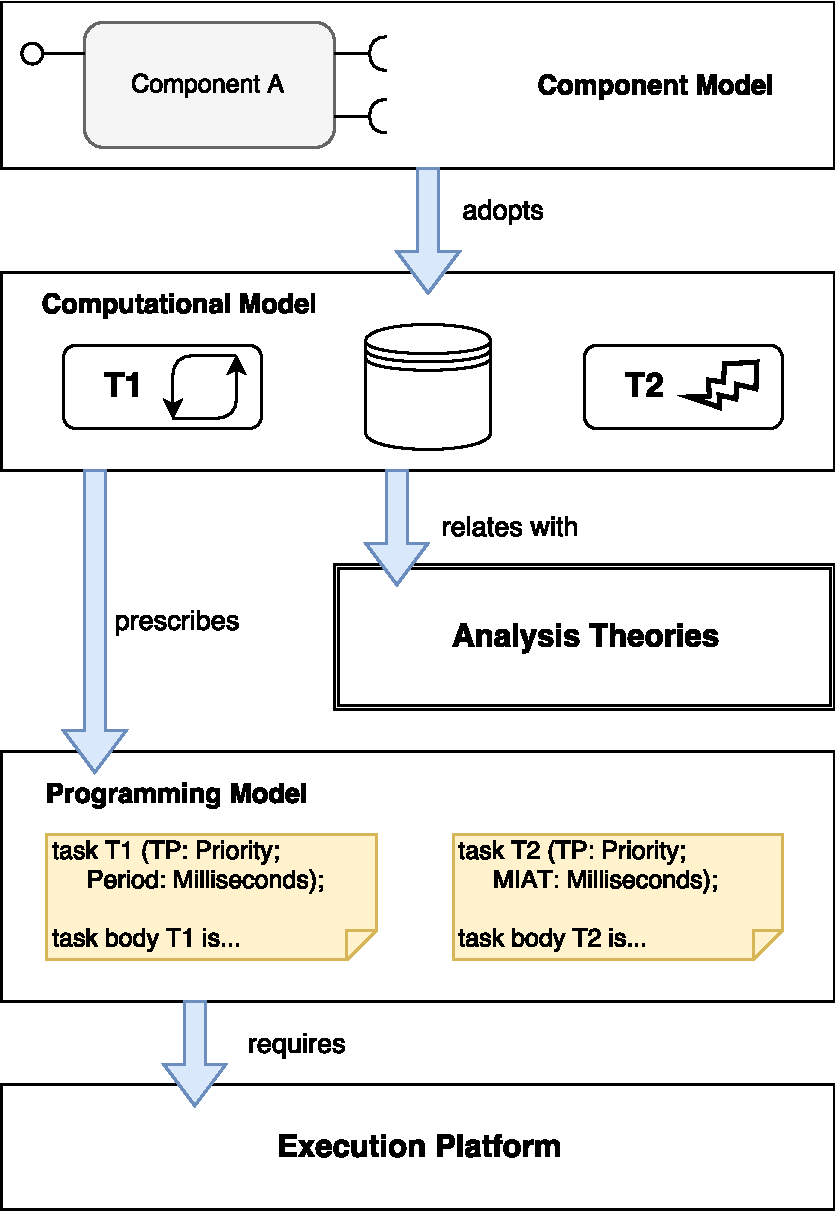
\includegraphics[width=0.5\textwidth]{ConstituentsOfSWArchitecture.pdf}
	\caption{The four constituents of the software reference architecture}
	\source{\cite{PhdThesis}}
	\label{fig: Constituents of OSRA}
\end{figure}

\subsection{Component Model}
\ac{cbse} is a software methodology centered on the systematic re-use of software by realizing the software as assembly of units of composition called components \cite{CBSE}.
The adoption of Component Based Software Engineering (CBSE) in the context of high-integrity real-time systems in general and in space domain in particular is not so popular as in the other main-stream domains like enterprise computing \cite{SAVOIR} because of strong verification and validation requirements imposed in the space domain and the presence of non-functional dimensions \cite{SAVOIR}.

The principles of Component Based Software Engineering (CBSE) when combined with the principles below can be used to build OBSW as an assembly of components \cite{SAVOIR}: 
\begin{itemize}
\item Principle of separation of concerns, by allocation of concerns to three distinct software entities: the component (which is a design entity), the container and the connector (which are entities used in implementation only and do not appear in the design space)
\item Possibility of verification of properties related to composability and compositionality \cite{CompBasedDev} 
\end{itemize}

The execution platform defined in the software architecture then provides the services to the components, container and the connectors. Finally, the entire software is deployed on the physical architecture (Computational units, equipment, and the network interconnections between them).

\subsubsection{\textbf{Founding principles of choice}}
This section describes the founding principles of choice of the component model:

\begin{description}
\item[Correctness by construction] E.W. Dijkstra in his ACM Turing lecture in 1972 suggested that the program construction should be done after a valid proof of correctness of construction has been developed \cite{CompBasedProcess}. Two decades later, a software development approach called Correctness by Construction (C-by-C) was proposed which advocated the detection and removal of errors at early stages, which leads to safer, cheaper and more reliable software \cite{CompBasedProcess}\cite{PhdThesis}. The Correctness by Construction practice follows:
\begin{itemize}
\item To give a solid reasoning on the correctness of the document or code, it is necessary to use formal and precise tools and notations for their development and verification 
\item Defining things only once so as to avoid contradictions and repetitions
\item Designing the software that is easy to verify e.g. by using safer language subsets or using appropriate coding styles and software design patterns. 
\end{itemize}

In OSRA and the component model developed along with it, the Correctness by Construction principle is changed to be applicable to a CBSE approach based on Model-driven Engineering (MDE) \cite{CompBasedProcess} wherein:

\begin{itemize}
\item The components are designed
\item The products designed by the design environment can be verified and analyzed by the design environment.
\item The lower level artifacts are automatically generated and the software production is automated to the maximum extent.  
\end{itemize}

\item [Separation of concerns] 
\label{section: Founding principle-Separation of concerns} 
Separation of concerns was first advocated by Dijkstra \cite{CompBasedProcess} and it helps to separate the aspects of software design and implementation. The OSRA and its associated component model promotes separation of concerns\cite{CompBasedProcess}\cite{PhdThesis}:

\begin{itemize}
\item The components are restricted to hold the functional code only. The non-functional requirements which has effects on the run-time behavior e.g. tasking, synchronization and timing are dealt by the component infrastructure, which is external to the component which realizes the functional code. The component infrastructure mainly consists of containers, connectors and their run-time support.

\item A specific annotation language is specified which is used to define the non-functional requirements and these are annotated on the components realizing the functional code.

By this, model transformations that automatically produce the containers and connectors that serve the non-functional requirements, enable the execution of the schedulability analysis directly on the model of components. This makes the implementation of the non-functional concerns fully compliant with its specification \cite{ScheduAnaly}. 

\item A code generator (whose development is the prime concern of this Master thesis) operates in the back-end of the component model, builds all of the component infrastructure that embeds the user components, their assemblies and the component services that help satisfy the non-functional properties \cite{CharEvoRAVCodeAr}. 
\end{itemize}

Inculcating the principle of separation of concerns in the development process has two major benefits \cite{CompBasedProcess}:

\begin{itemize}
\item It increases the reuse potential of the components, which is an important high level requirement described in the previous section \cite{SAVOIR}. The reuse potential of the component is increased because the same component can now be used under different non-functional requirements (as per the instantiations of the component infrastructure).

\item It helps in the generation of vast amount of complex and delicate infrastructural code which takes care of realizing the non-functional requirements on the run-time behavior of the software. This increases the readability, traceability and maintainability of the infrastructural code. 
\end{itemize}

\item [Composition] 
\label{section: Founding principle-Composition}
When composability and compositionality can be assured by static analysis, guaranteed through implementation, actively preserved at run-time, the goal of composition with guarantees as discussed by Vardanega can be achieved \cite{CompBasedProcess}. This is also one of the high level requirements defined in the section before.
 
Composability is guaranteed when the properties of individual components are preserved on component composition, deployment on target and execution. The components, as mentioned before, implement functional code, most part of which is sequential only and they do not have to worry about the non-functional semantics. The components behave like black-boxes and showcase to the external world only provided and required interfaces. Other components or infrastructural components are expected to communicate through these defined interfaces only. Hence, when components are composed with each other with matching required and provided interfaces, the functional composability is guaranteed which is necessary but not sufficient.

The non-functional requirements/constraints are annotated on the components (specifically the component interfaces) and they are realized by the container which encapsulates the respective component \cite{SAVOIR}\cite{ComponentModel}. The provided interface determines the semantics of the invocation and adds to the functional capabilities provided by the component. These semantics must match with the execution semantics described by the computational model, to which the component model is attached. An example for composable property is shown in \cref{fig: Composability}. In this case, the number of threads and protected objects generated per component, which entirely depends on the extra functional notations to the component interface should be invariant across component composition for the composable property to hold true.  

\begin{figure}[h]
	\centering
	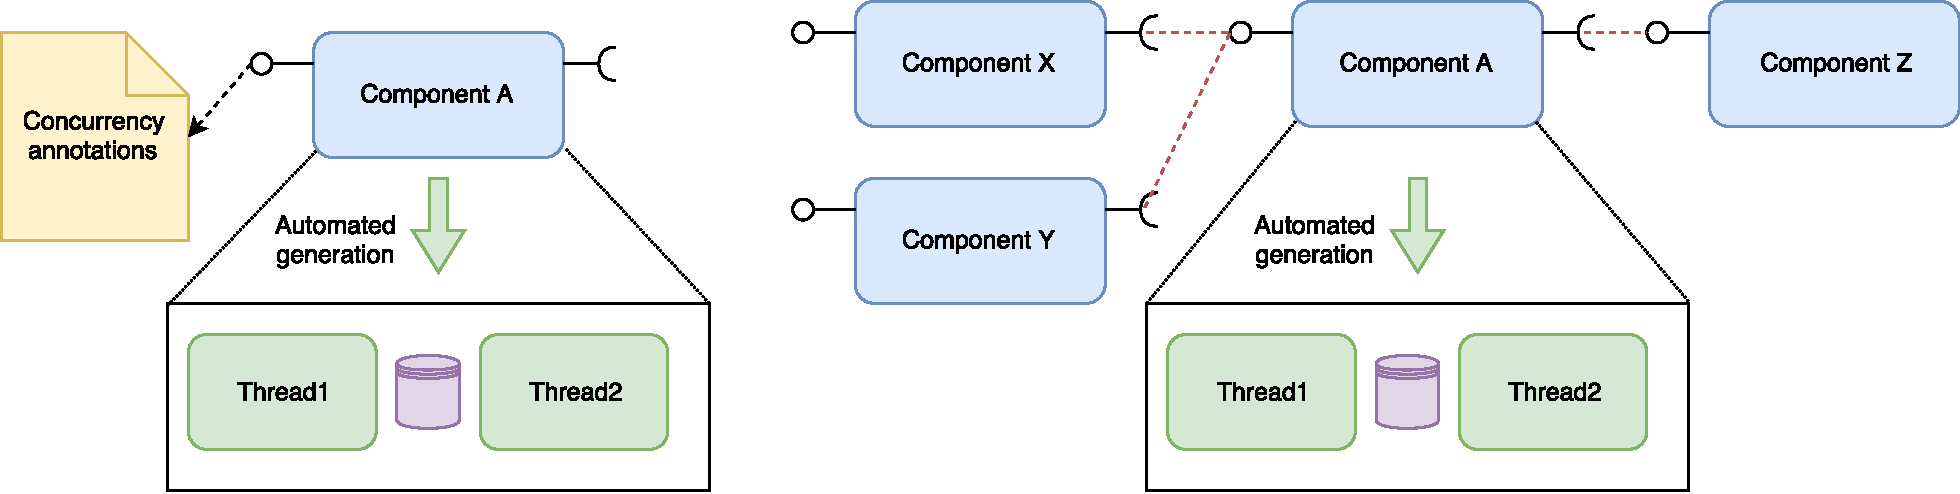
\includegraphics[width=1.0\textwidth]{Composability.pdf}
	\caption{Example for composability}
	\source{\cite{PhdThesis}}
	\label{fig: Composability}
\end{figure}

The computational model chosen should help extend composability to the non-functional constraints e.g. concurrency and the ones related to real-time and make it possible to get a compositional view of how execution occurs at the system level. Compositionality is said to be achieved when the properties of the system as a whole is a function of the properties of the constituting components. Finally, the binding of the computational model to the component should allow the execution semantics of the components with non-functional descriptors to be completely understood. An example for compositionality in shown in \cref{fig: Compositionality}. In this case, it should be possible to calculate the overall latency for the delivery of an output (i.e., the worst-case response time of the end-to-end chain of activities) from individual latencies of different components for the property of compositionality to hold true.

\begin{figure}[h]
	\centering
	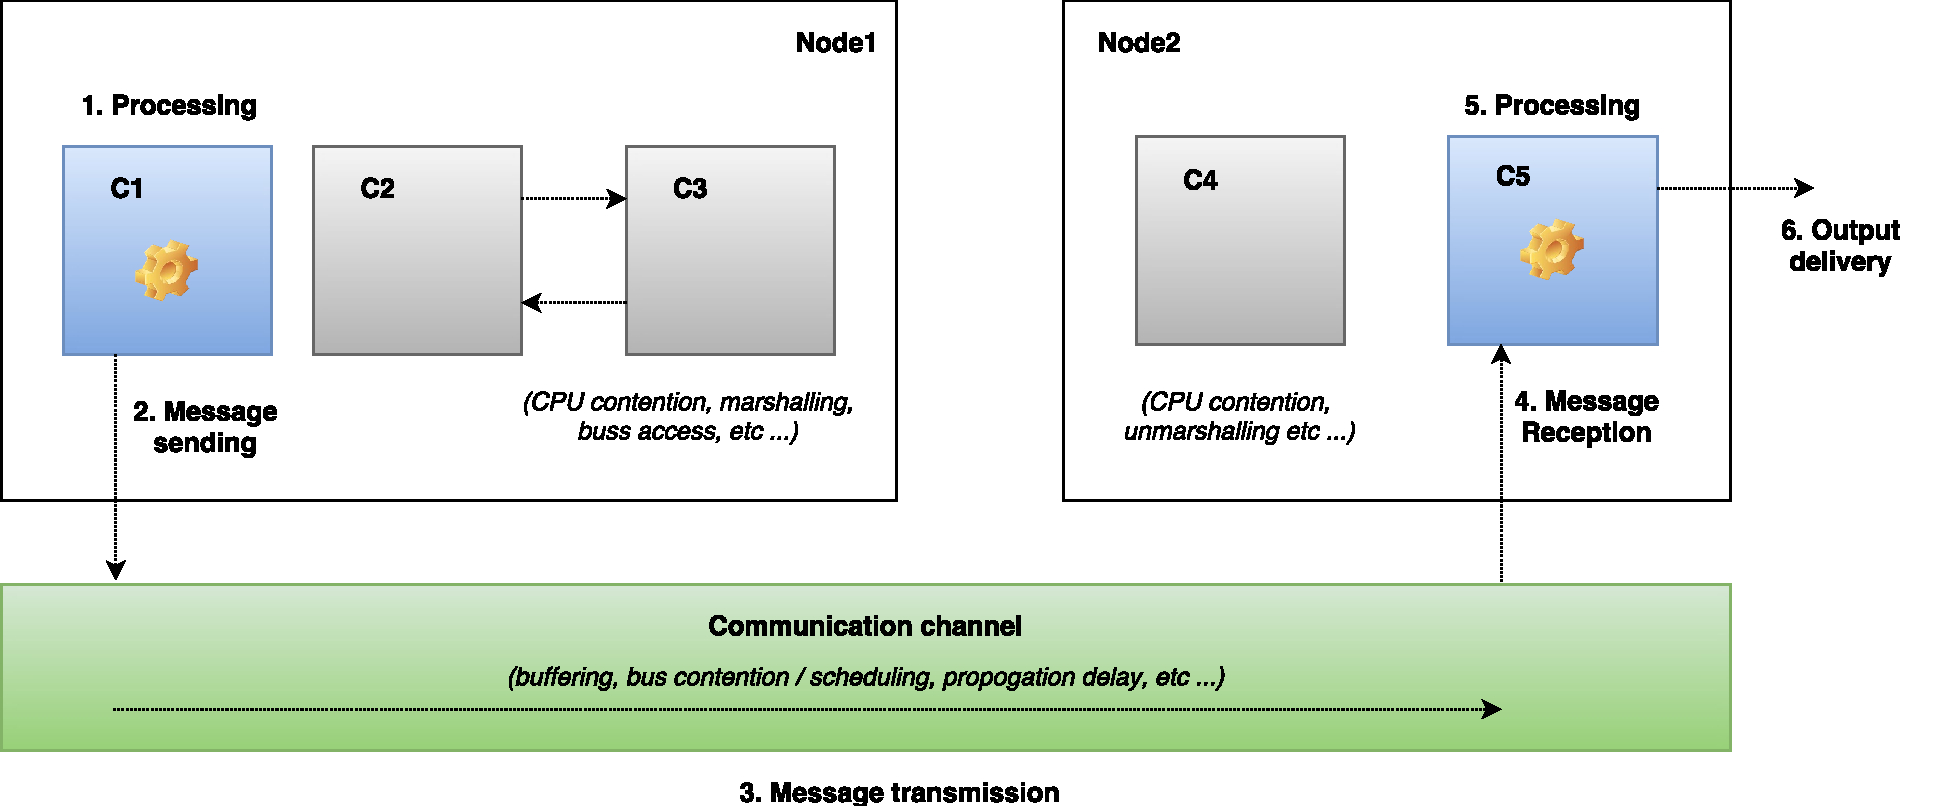
\includegraphics[width=1.0\textwidth]{Compositionality.pdf}
	\caption{Example for compositionality}
	\source{\cite{PhdThesis}}
	\label{fig: Compositionality}
\end{figure} 

In OSRA, the first and second needs can be met by having correct representations of the non-functional attributes in the component interfaces and the third need is taken care of by the generation of proper code artifacts, which is the main concern of this Master thesis.     
\end{description}

\subsubsection{\textbf{Software entities}}
\label {section: Software entities}
The following section describes more about components, containers and the connectors.

\begin{description}
\item[Component] Chaudron and Crnkovic describe that a Component model defines standards for properties that individual components must satisfy and the methods and possibly ways to compose components \cite{CompBasedProcess}.

A component provides a set of services and exposes them to the external world as a "provided interface". The service which is needed from other components or the environment in general are declared in a "required interface". A particular component connects to other components in order to satisfy the needs of its required interfaces. An event based communication system is also possible between components and a component can register to an "event service" to get notified about events emitted by other components.

Non functional attributes are added to the component interfaces as discussed before in the previous section on separation of concerns.

The adoption of hierarchical decomposition of components can be an effective way of defining components instead of defining a containment relationships. A child component can be developed to any component which would delegate and subsume the relationships between the interfaces of the child component and its parent. But the drawback is that various non-functional dimensions applicable to the space domain complicate the picture and hence is hierarchical decomposition of components not allowed at the current stage pf development \cite{PhdThesis}.
    
\item [Container] The container is a software entity that wraps around the component, which is directly responsible for realizing the non-functional properties. The relation between the component and the container is a famous software design pattern called the "inversion of control" \cite{CompBasedProcess}\cite{InvOfCntrlurl}. All in all, the reusable code (the container), controls the execution of the problem-specific code (the component).

The container exposes the same provided and required interfaces as that of the component and is able to support the component's execution with the desired, relevant non functional concerns attached to the component interface \cite{CompBasedDev}. The container also intercepts the calls made by the component to the other components/services requested from the target platform and transparently forward them to the container of the target component/target platform pseudo component (A pseudo component is a kind of component which is used for interaction purposes only). The former principle is called interface "promotion" and the latter is called the interface "subsumption" \cite{CompBasedDev}. The container and the component interact with each other according to the inversion of control design pattern, but the binding between components are still defined at software initialization time.

\item [Connector] The connector is a software entity responsible for the interaction between the components (actually between the containers that wrap around them). Connectors assist in implementing separation of concerns as the concerns of interaction is separated from the functional concerns. Components are thus void of code related to interactions with other components, however the the component model requires that the user specifies the interaction style in the component interfaces.

The component can be specified independently of the components it eventually binds to, the cardinality of the communication and the location of the other components it connects to, thanks to the principle of separation of concerns. 

No complex connectors are necessary in this Master thesis because, a simple linux based PC is chosen as a target system for component deployment and this greatly reduces the variety of connectors needed. Connectors necessary for function/procedure calls (which are usually straight-forward) are sufficient in this Master thesis. One of the major reasons, to go for a simple system is because this Master thesis does not deal with the hardware design or hardware modeling of the on-board software systems.           
\end{description} 

\cref{fig: Components containers and connectors} shows a connector mediating a connection between components A and B. The figure also shows components A and B being enveloped by their containers respectively. The containers would be responsible for the realization of the non-functional properties of the respective components they envelop. 

\begin{figure}[h]
	\centering
	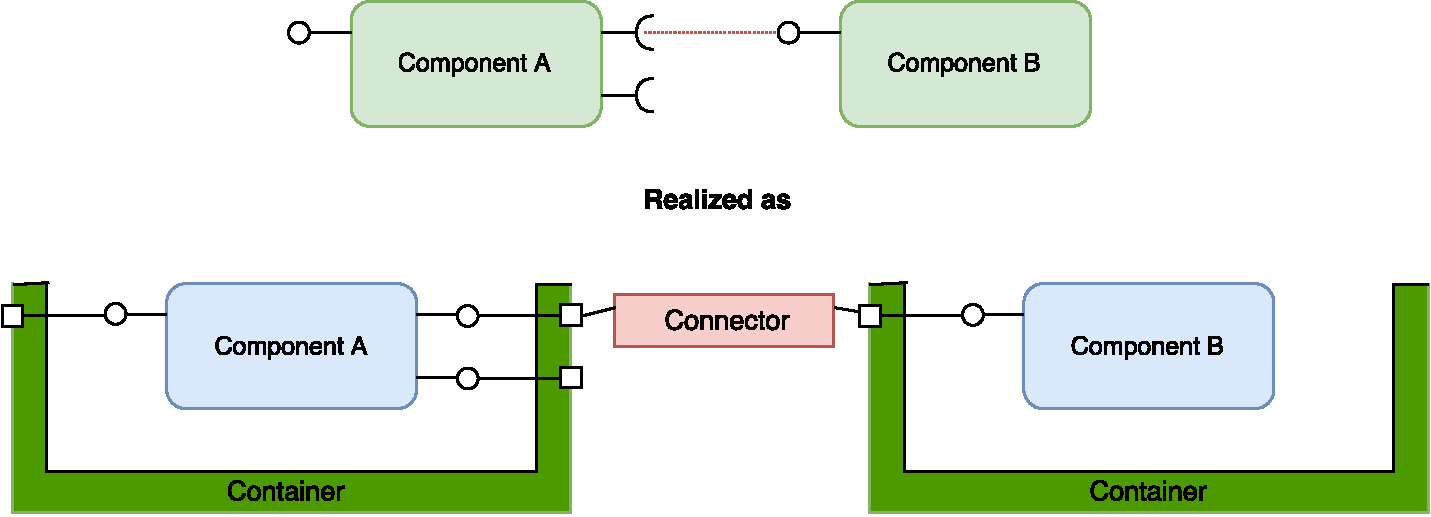
\includegraphics[width=0.8\textwidth]{ComponentContainerConnector.pdf}
	\caption{Components, containers and a connector connecting them}
	\source{\cite{SpecMetamodel}}
	\label{fig: Components containers and connectors}
\end{figure} 

\subsection{Computational model}
\label{section: Computational model} 
Using a computational model is necessary as per the Space Software engineering standard (ECSS-E-ST-440C) standard \cite{SAVOIR}. A dynamic software architecture is described according to an analyzable computational model which infers that the model development is fully consistent with that which underpins the mathematical equations which are used to predict the schedulability behavior of the system \cite{ScheduAnaly}. The computational model is more concerned about entities that belong to the implementation model (eg. tasks, protected objects and semaphores). A more abstract level description of these entities should be provided so that \cite{SAVOIR}:

\begin{itemize}
\item Pollution of the user-models with entities that are more primitive and are of interest to the lower levels of abstraction, is avoided. This is in line with the principle of separation of concerns, which is one of the high-level requirements.

\item The abstract representations represent the entities and their semantics faithfully.

\item Correct transformation of the information set by the designer in the higher-level representation to entities recognized by the computational model is ensured. This is in line with the principle of property preservation, which is also one of the high level requirements. 
\end{itemize} 

\subsection{Programming model and the execution platform}
\label{section: Execution platform}
The execution platform is a part of the software architecture providing all the necessary means for the implementation of a component and the computational model. It comprises of the middleware, the \ac{rtos}/\ac{rtk}, communication drivers and the board support package (BSP) for a given hardware platform. The services provided by the execution platform can be categorized into four different types \cite{SAVOIR}:

\begin{description}
\item [Services for containers] These services are meant to be used by the containers e.g. Tasking primitives, synchronization primitives, primitives related to time and timers.

\item [Services for connectors] These services are intended to be used by the connectors and it consists of actual communication means between components, ways to handle physical distribution across processing units, libraries used for translating data codes.

\item [Services to components] These services are supposed to be used by the components which implement the functional constraints. Typical services include: provision of on-board time for time-stamps, context management and data recovery. Access to these services are intercepted by the container wrapped around the component (refer section \cref{section: Software entities})

\item [Services to implement "abstract components"] These services include PUS monitoring, OBCPs, hardware representation etc.
\end{description}

It is important to note that different implementation of containers and connectors are necessary for each execution platform of interest.

The programming model realizes a given computational model and together with a conforming execution platform, it is possible to achieve the following goals \cite{PhdThesis}:

\begin{itemize}
\item Ensure that the implementation fully conforms with the semantics prescribed by the computational model and those assumed by the analysis
\item Ensure that the contracts stipulated between the components are respected at run-time. This is in-line with the principle of property preservation which is one of the high level requirements.
\end{itemize} 

The achievement of those two goals would then warrant that the system represented for the analysis purposes is a faithful representation of its implementation and the results of the analysis performed on the system model would be a valid prediction of the system at run-time \cite{PhdThesis}.

The programming model, which is the subject of this Master thesis, is realized by adopting Tasking framework as a computational model whose concurrency semantics would conform to the analysis model.     

% !TeX spellcheck = en_US

\chapter{Results and Conclusions}
\label{chap:conclusion}

\section{Discussion}
As a part of this Master thesis, 
\begin{itemize}
\item A choice is made to use the Tasking framework as a computational model so that the OSRA component model statically binds to Tasking framework which formally defines the computational entities and the rules which govern their usage 
\item A reference programming model is decided upon that enforces the analysis assumptions and which permits to express exclusively the semantics imposed by the analysis theory and which conveys the implementations of the desired non-functional properties using the primitives from the Tasking framework
\item Different corner cases which might arise during the construction of an OBSW model using the OSRA component model are identified 
\item An overall software design approach for the generated infrastructure code of the OBSW models is presented and a mapping of the OBSW model design entities to the infrastructural code entities is presented. The generated code would then have all the good characteristics of a software as listed in \cref{subsection: Software design approach} 
\item A code generator is implemented, using which the generation of the entire non-functional code i.e., the code for handling the concurrency and interaction requirements for communication between components and generation of component containers and component connectors can be automated. The code generator uses the already tried and tested Tasking framework as the platform and bases the generated code on it. The advantage of this is that it eases the model-to-code transformation step 
\item The implemented code generator is tested for multiple OBSW models as shown in \cref{chap: Extra examples} which capture the different corner cases identified
\item For the simple OBSW model example which was introduced in \cref{chap: Code generation}, a set of unit test cases are written using Gtest and Gmock frameworks and the test coverage reports are generated
\end{itemize}

The following results were obtained 
\begin{itemize}
\item  The implemented code generator successfully generates the infrastructural code entities for all the example OBSW models listed in \cref{chap: Code generation} and in \cref{chap: Extra examples}. The generated code in all cases is successfully compiled along with Tasking framework using GCC C++ compiler conforming to the C++11 standard for the Linux platform
\item The test coverage reports generated for the unit tests written for the simple OBSW example are analyzed. The results show that the testability factor of the generated code is high and the infrastructural code entities can be efficiently tested      
\end{itemize}

\section{Identified shortcomings of Tasking framework}
During the course of the Master thesis, the following shortcomings of the current version of Tasking framework, which is chosen as a computational model for this Master thesis are identified:
\begin{itemize}
\item Tasks from Tasking framework are used in various threads of control as explained in \cref{chap: Progamming model}. At the heart of the Tasking framework is a scheduler which schedules tasks based on priorities and these tasks are non-preemptible at the moment \cite{TaskFr}. This is one of the critical shortcomings in the current version of the Tasking framework as it makes the generated software code which is based on Tasking framework not suitable for hard real-time systems \cite{TempIsolation}. Time-monitoring architectures such as Server-based architecture or Priority-Band architectures listed in \cite{TempIsolation} are the ways to go ahead in case making the code making use of the Tasking framework truly real-time capable. These architectures help in providing isolation of applications i.e., tasks (at least) along three orthogonal dimensional axes: time, space and communication
\item In the current version of the Tasking framework there is no possibility to measure the run-time of the tasks and monitor deadline violations which are mostly caused by WCET overruns of either the task at hand or a higher priority task. This limits the extent of property preservation in the model-to-code transformation step \cite{TempIsolation}. It is of very high importance that the system properties asserted during the analysis and the assumptions made for the analysis to hold are preserved across implementation and execution \cite{EvoRAVCodeAr}\cite{TempIsolation}
\item It is also not possible to measure the execution time of a group tasks which are associated to the single time budget so that the Group Budget is accounted for their collective execution time. This incapability makes the adoption of Server-based architecture in the Tasking framework more difficult
\item In line with the inability to measure the run-time of the tasks from the Tasking framework, Tasking Framework also does not provide any constructs for at least coarse-grained fault detection and fault handling in case of deadline misses
\item 
\end{itemize}

\section{Future Work}
As an enhancement to the current work, it is possible to extend this Master thesis  
\label{section: Future work}


%
%
%\renewcommand{\appendixtocname}{Anhang}
%\renewcommand{\appendixname}{Anhang}
%\renewcommand{\appendixpagename}{Anhang}
\appendix
$  $% !TeX spellcheck = de_DE
%Die Angabe des schlauen Spruchs auf diesem Wege funtioniert nur,
%wenn keine Änderung des Kapitels mittels den in preambel/chapterheads.tex
%vorgeschlagenen Möglichkeiten durchgeführt wurde.
\setchapterpreamble[u]{%
\dictum[Albert Einstein]{Probleme kann man niemals mit derselben Denkweise lösen, durch die sie entstanden sind.}
}
\chapter{LaTeX-Tipps}
\label{chap:latextipps}

\section{File-Encoding und Unterstützung von Umlauten}
\label{sec:firstsectioninlatexhints}
Die Vorlage wurde 2010 auf UTF-8 umgestellt.
Alle neueren Editoren sollten damit keine Schwierigkeiten haben.

\section{Zitate}
Referenzen werden mittels \texttt{\textbackslash cite[key]} gesetzt.
Beispiel: \cite{WSPA} oder mit Autorenangabe: \citet{WSPA}.

Der folgende Satz demonstriert \begin{inparaenum}[1.]
\item die Großschreibung von Autorennamen am Satzanfang,
\item die richtige Zitation unter Verwendung von Autorennamen und der Referenz,
\item dass die Autorennamen ein Hyperlink auf das Literaturverzeichnis sind sowie
\item dass in dem Literaturverzeichnis der Namenspräfix \enquote{van der} von \enquote{Wil M.\,P.\ van der Aalst} steht.
\end{inparaenum}
\Citet{RVvdA2016} präsentieren eine Studie über die Effektivität von Workflow-Management-Systemen.

Der folgende Satz demonstriert, dass man mittels \texttt{label} in einem Bibliopgrahie"=Eintrag den Textteil des generierten Labels überschreiben kann, aber das Jahr und die Eindeutigkeit noch von biber generiert wird.
Die Apache ODE Engine \cite{ApacheODE} ist eine Workflow-Maschine, die BPEL-Prozesse zuverlässig ausführt.

Wörter am besten mittels \texttt{\textbackslash enquote\{...\}} \enquote{einschließen}, dann werden die richtigen Anführungszeichen verwendet.

Beim Erstellen der Bibtex-Datei wird empfohlen darauf zu achten, dass die DOI aufgeführt wird.

\section{Mathematische Formeln}
\label{sec:mf}
Mathematische Formeln kann man $so$ setzen. \texttt{symbols-a4.pdf} (zu finden auf \url{http://www.ctan.org/tex-archive/info/symbols/comprehensive/symbols-a4.pdf}) enthält eine Liste der unter LaTeX direkt verfügbaren Symbole.
Z.\,B.\ $\mathbb{N}$ für die Menge der natürlichen Zahlen.
Für eine vollständige Dokumentation für mathematischen Formelsatz sollte die Dokumentation zu \texttt{amsmath}, \url{ftp://ftp.ams.org/pub/tex/doc/amsmath/} gelesen werden.

Folgende Gleichung erhält keine Nummer, da \texttt{\textbackslash equation*} verwendet wurde.
\begin{equation*}
x = y
\end{equation*}

Die Gleichung~\ref{eq:test} erhält eine Nummer:
\begin{equation}
\label{eq:test}
x = y
\end{equation}

Eine ausführliche Anleitung zum Mathematikmodus von LaTeX findet sich in \url{http://www.ctan.org/tex-archive/help/Catalogue/entries/voss-mathmode.html}.

\section{Quellcode}
\Cref{lst:ListingANDlstlisting} zeigt, wie man Programmlistings einbindet.
Mittels \texttt{\textbackslash lstinputlisting} kann man den Inhalt direkt aus Dateien lesen.

%Listing-Umgebung wurde durch \newfloat{Listing} definiert
\begin{Listing}
\begin{lstlisting}
<listing name="second sample">
  <content>not interesting</content>
</listing>
\end{lstlisting}
\caption{lstlisting in einer Listings-Umgebung, damit das Listing durch Balken abgetrennt ist}
\label{lst:ListingANDlstlisting}
\end{Listing}

Quellcode im \lstinline|<listing />| ist auch möglich.

\section{Abbildungen}

Die \cref{fig:chor1} und \ref{fig:chor2} sind für das Verständnis dieses Dokuments wichtig.
Im Anhang zeigt \vref{fig:AnhangsChor} erneut die komplette Choreographie.

%Die Parameter in eckigen Klammern sind optionale Parameter - z.B. [htb!]
%htb! bedeutet: "Liebes LaTeX, bitte platziere diese Abbildung zuerst hier ("_h_ere"). Falls das nicht funktioniert, dann bitte oben auf der Seite ("_t_op"). Und falls das nicht geht, bitte unten auf der Seite ("_b_ottom"). Und bitte, bitte bevorzuge hier und oben, auch wenn's net so optimal aussieht ("!")
%Diese sollten nach Möglichkeit NICHT verwendet werden. LaTeX's Algorithmus für das Platzieren der Gleitumgebung ist schon sehr gut!
\begin{figure}
  \centering
  \includegraphics[width=\textwidth]{choreography.pdf}
  \caption{Beispiel-Choreographie}
  \label{fig:chor1}
\end{figure}

\begin{figure}
  \centering
  \includegraphics[width=.8\textwidth]{choreography.pdf}
  \caption[Beispiel-Choreographie]{Die Beispiel-Choreographie. Nun etwas kleiner, damit \texttt{\textbackslash textwidth} demonstriert wird. Und auch die Verwendung von alternativen Bildunterschriften für das Verzeichnis der Abbildungen. Letzteres ist allerdings nur Bedingt zu empfehlen, denn wer liest schon so viel Text unter einem Bild? Oder ist es einfach nur Stilsache?}
  \label{fig:chor2}
\end{figure}


\begin{figure}
  \centering
    \subfloat[]{\includegraphics[width=0.3\textwidth]{choreography.pdf} \label{fig:subfigA}}
    \subfloat[]{\includegraphics[width=0.3\textwidth]{choreography.pdf} \label{fig:subfigB}}
		\subfloat[Subcaption if needed]{\includegraphics[width=0.3\textwidth]{choreography.pdf} \label{fig:subfigC}}
	\caption{Beispiel um 3 Abbildung nebeneinader zu stellen nur jedes einzeln referenzieren zu können. Abbildung~\ref{fig:subfigB}
 ist die mittlere Abbildung.}
\label{fig:subfig_example}
\end{figure}

Das SVG in \cref{fig:directSVG} ist direkt eingebunden, während der Text im SVG in \cref{fig:latexSVG} mittels pdflatex gesetzt ist.
\todo{Falls man die Graphiken sehen möchte, muss inkscape im PATH sein und im Tex-Quelltext \texttt{\textbackslash{}iffalse} und \texttt{\textbackslash{}iftrue} auskommentiert sein.}

\iffalse % <-- Das hier wegnehmen, falls inkscape im Pfad ist
\begin{figure}
\centering
\includegraphics{svgexample.svg}
\caption{SVG direkt eingebunden}
\label{fig:directSVG}
\end{figure}

\begin{figure}
\centering
\def\svgwidth{.4\textwidth}
\includesvg{svgexample}
\caption{Text im SVG mittels \LaTeX{} gesetzt}
\label{fig:latexSVG}
\end{figure}
\fi % <-- Das hier wegnehmen, falls inkscape im Pfad ist

\section{Tabellen}

\cref{tab:Ergebnisse} zeigt Ergebnisse und die \cref{tab:Ergebnisse} zeigt wie numerische Daten in einer Tabelle representiert werden können.
\begin{table}
  \centering
  \begin{tabular}{ccc}
  \toprule
  \multicolumn{2}{c}{\textbf{zusammengefasst}} & \textbf{Titel} \\ \midrule
  Tabelle & wie & in \\
  \url{tabsatz.pdf}& empfohlen & gesetzt\\

  \multirow{2}{*}{Beispiel} & \multicolumn{2}{c}{ein schönes Beispiel}\\
   & \multicolumn{2}{c}{für die Verwendung von \enquote{multirow}}\\
  \bottomrule
  \end{tabular}
  \caption[Beispieltabelle]{Beispieltabelle -- siehe \url{http://www.ctan.org/tex-archive/info/german/tabsatz/}}
  \label{tab:Ergebnisse}
\end{table}

\begin{table}
	\centering
	\begin{tabular}{l *{8}{d{3.2}}}
		\toprule
						
			   & \multicolumn{2}{c}{\textbf{Parameter 1}} & \multicolumn{2}{c}{\textbf{Parameter 2}} & \multicolumn{2}{c}{\textbf{Parameter 3}} & \multicolumn{2}{c}{\textbf{Parameter 4}} \\
			\cmidrule(r){2-3}\cmidrule(lr){4-5}\cmidrule(lr){6-7}\cmidrule(l){8-9}
			
			\textbf{Bedingungen} & \multicolumn{1}{c}{\textbf{M}} & \multicolumn{1}{c}{\textbf{SD}} & \multicolumn{1}{c}{\textbf{M}} & \multicolumn{1}{c}{\textbf{SD}} & \multicolumn{1}{c}{\textbf{M}} & \multicolumn{1}{c}{\textbf{SD}} & \multicolumn{1}{c}{\textbf{M}} & \multicolumn{1}{c}{\textbf{SD}}\\
			\midrule
			
			W & 1.1 & 5.55 & 6.66 & .01 &  &  &  & \\
			X & 22.22 & 0.0 & 77.5 & .1 &  &  &  & \\
			Y & 333.3 & .1 & 11.11 & .05 &  &  &  & \\
			Z & 4444.44 & 77.77 & 14.06 & .3 &  &  &  & \\
		\bottomrule 
	\end{tabular}
	
	\caption{Beispieltabelle f\"{u}r 4 Bedingungen (W-Z) mit jeweils 4 Parameters mit (M und SD). Hinweiß: immer die selbe anzahl an Nachkommastellen angeben.}
	\label{tab:Werte}
\end{table}

\section{Pseudocode}
\Cref{alg:sample} zeigt einen Beispielalgorithmus.
\begin{Algorithmus} %Die Umgebung nur benutzen, wenn man den Algorithmus ähnlich wie Graphiken von TeX platzieren lassen möchte
\caption{Sample algorithm}
\label{alg:sample}
\begin{algorithmic}
\Procedure{Sample}{$a$,$v_e$}
\State $\mathsf{parentHandled} \gets (a = \mathsf{process}) \lor \mathsf{visited}(a'), (a',c,a) \in \mathsf{HR}$
\State \Comment $(a',c'a) \in \mathsf{HR}$ denotes that $a'$ is the parent of $a$
\If{$\mathsf{parentHandled}\,\land(\mathcal{L}_\mathit{in}(a)=\emptyset\,\lor\,\forall l \in \mathcal{L}_\mathit{in}(a): \mathsf{visited}(l))$}
\State $\mathsf{visited}(a) \gets \text{true}$
\State $\mathsf{writes}_\circ(a,v_e) \gets
\begin{cases}
\mathsf{joinLinks}(a,v_e) & \abs{\mathcal{L}_\mathit{in}(a)} > 0\\
\mathsf{writes}_\circ(p,v_e)
& \exists p: (p,c,a) \in \mathsf{HR}\\
(\emptyset, \emptyset, \emptyset, false) & \text{otherwise}
\end{cases}
$
\If{$a\in\mathcal{A}_\mathit{basic}$}
  \State \Call{HandleBasicActivity}{$a$,$v_e$}
\ElsIf{$a\in\mathcal{A}_\mathit{flow}$}
  \State \Call{HandleFlow}{$a$,$v_e$}
\ElsIf{$a = \mathsf{process}$} \Comment Directly handle the contained activity
  \State \Call{HandleActivity}{$a'$,$v_e$}, $(a,\bot,a') \in \mathsf{HR}$
  \State $\mathsf{writes}_\bullet(a) \gets \mathsf{writes}_\bullet(a')$
\EndIf
\ForAll{$l \in \mathcal{L}_\mathit{out}(a)$}
  \State \Call{HandleLink}{$l$,$v_e$}
\EndFor
\EndIf
\EndProcedure
\end{algorithmic}
\end{Algorithmus}

\clearpage
Und wer einen Algorithmus schreiben möchte, der über mehrere Seiten geht, der kann das nur mit folgendem \textbf{üblen} Hack tun:

{
\begin{minipage}{\textwidth}
\hrule height .8pt width\textwidth
\vskip.3em%\vskip\abovecaptionskip\relax
\stepcounter{Algorithmus}
\addcontentsline{alg}{Algorithmus}{\protect\numberline{\theAlgorithmus}{\ignorespaces Description \relax}}
\noindent\textbf{Algorithmus \theAlgorithmus} Description
%\stepcounter{algorithm}
%\addcontentsline{alg}{Algorithmus}{\thealgorithm{}\hskip0em Description}
%\textbf{Algorithmus \thealgorithm} Description
\vskip.3em%\vskip\belowcaptionskip\relax
\hrule height .5pt width\textwidth
\end{minipage}
%without the following line, the text is nerer at the rule
\vskip-.3em
%
code goes here\\
test2\\
%
\vskip-.7em
\hrule height .5pt width\textwidth
}


\section{Abkürzungen}

Beim ersten Durchlaf betrug die \ac{FR} 5. Beim zweiten Durchlauf war die \ac{FR} 3.

Mit \verb+\ac{...}+ können Abkürungen eingebaut werden, beim ersten aufrufen wird die lange Form eingesetzt. Beim wiederholten Verwenden von \verb+\ac{...}+ wird automatisch die kurz Form angezeigt. Außerdem wird die Abkürzung automatisch in die Abkürzungsliste eingefügt.

Definiert werden Abkürzungen in der Datei \textit{ausarbeitung.tex} im Abschnitt '\%\%\% acro' mithilfe von \verb+\DeclareAcronym{...}{...}+.

Mehr infos unter: \url{http://mirror.hmc.edu/ctan/macros/latex/contrib/acro/acro_en.pdf}

\section{Verweise}
Für weit entfernte Abschnitte ist \enquote{varioref} zu empfehlen:
\enquote{Siehe \vref{sec:mf}}.
Das Kommando \texttt{\textbackslash{}vref} funktioniert ähnlich wie \texttt{\textbackslash{}cref} mit dem Unterschied, dass zusätzlich ein Verweis auf die Seite hinzugefügt wird.
\texttt{vref}: \enquote{\vref{sec:firstsectioninlatexhints}}, \texttt{cref}: \enquote{\cref{sec:firstsectioninlatexhints}}, \texttt{ref}: \enquote{\ref{sec:firstsectioninlatexhints}}.

Falls \enquote{varioref} Schwierigkeiten macht, dann kann man stattdessen \enquote{cref} verwenden.
Dies erzeugt auch das Wort \enquote{Abschnitt} automatisch: \cref{sec:mf}.
Das geht auch für Abbildungen usw.
Im Englischen bitte \verb1\Cref{...}1 (mit großen \enquote{C} am Anfang) verwenden.


%Mit MiKTeX Installation ab dem 2012-01-16 nicht mehr nötig
%Falls ein Abschnitt länger als eine Seite wird und man mittels \texttt{\textbackslash{}vref} auf eine konkrete Stelle in der Section
%verweisen möchte, dann sollte man \texttt{\textbackslash{}phantomsection} verwenden und dann wird
%auch bei \texttt{vref} die richtige Seite angeben.

%%The link location will be placed on the line below.
%%Tipp von http://en.wikibooks.org/wiki/LaTeX/Labels_and_Cross-referencing#The_hyperref_package_and_.5Cphantomsection
%\phantomsection
%\label{alabel}
%Das Beispiel für \texttt{\textbackslash{}phantomsection} bitte im \LaTeX{}-Quellcode anschauen.

%Hier das Beispiel: Siehe Abschnitt \vref{hack1} und Abschnitt \vref{hack2}.

\section{Definitionen}
\begin{definition}[Title]
\label{def:def1}
Definition Text
\end{definition}

\Cref{def:def1} zeigt \ldots

\section{Verschiedenes}
\label{sec:diff}
\ifdeutsch
Ziffern (123\,654\,789) werden schön gesetzt.
Entweder in einer Linie oder als Minuskel-Ziffern.
Letzteres erreicht man durch den Parameter \texttt{osf} bei dem Paket \texttt{libertine} bzw.\ \texttt{mathpazo} in \texttt{fonts.tex}.
\fi

\textsc{Kapitälchen} werden schön gesperrt...

\begin{compactenum}[I.]
\item Man kann auch die Nummerierung dank paralist kompakt halten
\item und auf eine andere Nummerierung umstellen
\end{compactenum}

\section{Weitere Illustrationen}
Abbildungen~\ref{fig:AnhangsChor} und~\ref{fig:AnhangsChor2} zeigen zwei Choreographien, die den
Sachverhalt weiter erläutern sollen. Die zweite Abbildung ist um 90 Grad gedreht, um das Paket
\texttt{rotating} zu demonstrieren.

\begin{figure}
  \centering
  \includegraphics[width=\textwidth]{choreography.pdf}
  \caption{Beispiel-Choreographie I}
  \label{fig:AnhangsChor}
\end{figure}

\begin{landscape}
  %sidewaysfigure
  \begin{figure}
    \centering
    \includegraphics[width=\textwidth]{choreography.pdf}
    \caption{Beispiel-Choreographie II}
    \label{fig:AnhangsChor2}
  \end{figure}
\end{landscape}

\clearpage
%hint by http://tex.stackexchange.com/a/3265/9075
%other option is to use changepage according to http://tex.stackexchange.com/a/2639/9075. This, however, has issues with landscape
\thispagestyle{empty}

\savegeometry{koma}

%If you only have height problems, this is not needed at all
\addtolength{\textwidth}{2cm}
\addtolength{\evensidemargin}{-1cm}

\begin{landscape}
  %sidewaysfigure
  \begin{figure}
    \centerline{\includegraphics[width=0.9\paperheight]{choreography.pdf}}
    \caption{Beispiel-Choreographie, auf einer weißen Seite gezeigt wird und über die definierten Seitenränder herausragt}
  \end{figure}
\end{landscape}

%the original layout is restored.
%%\restoregeometry cannot be used as we use \addtolength
\loadgeometry{koma}

\section{Schlusswort}
Verbesserungsvorschläge für diese Vorlage sind immer willkommen.
Bitte bei github ein Ticket eintragen (\url{https://github.com/latextemplates/uni-stuttgart-computer-science-template/issues}).


%\printindex

\printbibliography

\ifdeutsch
Alle URLs wurden zuletzt am 17.\,03.\,2008 geprüft.
\else
All links were last followed on March 17, 2008.
\fi

\pagestyle{empty}
\renewcommand*{\chapterpagestyle}{empty}
\Versicherung
\end{document}
